\documentclass[../notes.tex]{subfiles}

\pagestyle{main}
\renewcommand{\chaptermark}[1]{\markboth{\chaptername\ \thechapter\ (#1)}{}}
\setcounter{chapter}{5}

\begin{document}




\chapter{???}
\section{Module Tools}
\begin{itemize}
    \item \marginnote{2/6:}A fifth week summary has been posted.
    \begin{itemize}
        \item Week 5 content is not in the midterm syllabus.
        \begin{itemize}
            \item In particular, Gauss's Lemma is not on the midterm.
        \end{itemize}
        \item Lecture 5.3 won't even be on the final syllabus.
        \item The techniques are applicable to a variety of problems, though, so it is good to know them.
    \end{itemize}
    \item Today: Modules.
    \begin{itemize}
        \item We depart from commutative rings and return to simple rings with identity to start.
    \end{itemize}
    \item Notation: What kinds of sets different letters denote.
    \begin{itemize}
        \item $A,B$: Rings.
        \item $R$: Commutative ring.
        \item $F,K$: Fields.
        \item $D$: Division ring.
    \end{itemize}
    \item Linear algebra is the study of division rings but only over fields.
    \item Definition of a \textbf{division ring}.
    \begin{itemize}
        \item The only ideals of a division ring are $0,D$, just like with fields.
        \item Linear independence, spanning, basis, etc. all hold in a general division ring; you only need fields for things like JCF.
    \end{itemize}
    \item \textbf{Left $\bm{A}$-module}: An abelian group $(M,+)$ equipped with a binary operation $\cdot:A\times M\to M$ defined by $(a,m)\mapsto am$ (or $a\cdot m$ in the case of potential ambiguity) satisfying the following. \emph{Constraints}\par
    For all $a,b\in A$ and $v,v_1,v_2\in M$\dots
    \begin{enumerate}[label={(\arabic*)}]
        \item $a(v_1+v_2)=av_1+av_2$;
        \item $(a+b)v=av+bv$;
        \item $a(bv)=(ab)v$;
        \item $1_Av=v$.
    \end{enumerate}
    \item We need the last one so that multiplication is nontrivial.
    \item A \textbf{right $\bm{A}$-module} puts the scalar on the right. Will we ever consider these??
    \item Notation: For all $a\in A$, define the function $\rho(a):M\to M$ by $\rho(a)v=av$ for all $v\in M$. \emph{Constraints}
    \begin{enumerate}[label={(\arabic*)}]
        \item $\rho(a)$ is a group homomorphism from $M\to M$.
        \item $\rho(a+b)=\rho(a)+\rho(b)$.
        \item $\rho(a)\rho(b)=\rho(ab)$.
        \item $\rho(1_A)=1_{\End(M)}$
    \end{enumerate}
    \item Conditions 2-4 imply that $\rho:A\to\End(M)$ is a ring homomorphism.
    \begin{itemize}
        \item Recall HW1 Q1.14, which led up to the result that
        \begin{equation*}
            \End(M) = \{f:M\to M\mid f\text{ is a group homomorphism}\}
        \end{equation*}
        is a ring with identity under componentwise addition and composition (i.e., $g\cdot f=g\circ f$).
    \end{itemize}
    \item Going forward, in-class definitions will always match those in the book.
    \begin{itemize}
        \item It's been this way for a while??
    \end{itemize}
    \item Examples.
    \begin{enumerate}
        \item Let $M=A$. Then $\rho(a)b=ab$ for all $a\in A$, $b\in M=A$.
        \item If $M_i$ ($i\in I$ an indexing set) is a (left) $A$-module, then the product $\prod_{i\in I}M_i$ is also an $A$-module.
        \item Denote an element of $\prod_{i\in I}M_i$ by $\prod_{i\in I}m_i$. An arbitrary choice of $m_i\in M_i$ for all $i\in I$ is allowed (do we need the Axiom of Choice??). We define $\cdot$ by
        \begin{equation*}
            a\left( \prod_{i\in I}m_i \right) = \prod_{i\in I}(am_i)
        \end{equation*}
        \item The collection
        \begin{equation*}
            \oplus_{i\in I}M_i = \left\{ \prod_{i\in I}m_i\mid\{i\in I:m_i\neq 0\}\text{ is a finite set} \right\}
        \end{equation*}
        is an $A$-module.
        \begin{itemize}
            \item This is a submodule of something??
            \item Under the same binary operation as Example 3??
        \end{itemize}
        \item In particular, $A^m$ is an $A$-module with $a(b_1,\dots,b_n)=(ab_1,\dots,ab_n)$.
    \end{enumerate}
    \item \textbf{Submodule}: A subgroup $(N,+)$ of $(M,+)$ such that for all $a\in A$ and $\omega\in N$, $a\omega\in N$.
    \item Observation: If $N_1,N_2$ are submodules of $M$, then $N_1+N_2$ and $N_1\cap N_2$ are submodules.
    \item Question (base case): What are the submodules of $A$, itself?
    \begin{itemize}
        \item Left ideals.
    \end{itemize}
    \item \textbf{Module homomorphism}: A function $T:M\to N$ such that $T$ is a homomorphism of abelian groups and commutes with scalar multiplication (i.e., $T(av)=aT(v)$ for all $a\in A$, $v\in M$). In full, we have
    \begin{equation*}
        T(a_1v_1+a_2v_2) = a_1T(v_1)+a_2T(v_2)
    \end{equation*}
    for all $a_1,a_2\in A$ and $v_1,v_2\in M$.
    \item Question: What are all of the module homomorphisms $T:A\to M$?
    \begin{itemize}
        \item If $T(1)=v$, then $T(a\cdot 1)=aT(1)=av$ for all $a\in A$.
        \item For all $v\in M$, there exists a unique $T:A\to M$ such that $T(1)=v$. This is more linear algebra.
    \end{itemize}
    \item Question: What are all linear transformations $T:A^n\to M$?
    \begin{itemize}
        \item Suppose $e_1=(1,0,\dots,0)$, $e_2=(0,1,0,\dots,0)$, etc. Then
        \begin{equation*}
            (a_1,\dots,a_n) = \sum_{i=1}^na_ie_i
        \end{equation*}
        \item Therefore,
        \begin{equation*}
            T(a_1,\dots,a_n) = \sum_{i=1}^na_iTe_i
        \end{equation*}
        \item Take any ordered $n$-tuple of elements in $M$; then given $v_1,\dots,v_n\in M$, there is a unique $A$-module homomorphism $T:A^n\to M$ such that $T(e_i)=v_i$ ($i=1,\dots,n$).
    \end{itemize}
    \item \textbf{Isomorphism} (of $A$-modules): A bijective module homomorphism $T:M\to N$, where $M,N$ are $A$-modules.
    \item It follows that $T^{-1}:N\to M$ is also a homomorphism.
    \item Proposition: Let $N$ be a submodule of $M$. Then the quotient group $M/N$ has a unique structure of an $A$-module such that $\pi:M\to M/N$ (defined with groups) is an $A$-module homomorphism.
    \begin{proof}
        {\color{white}hi}\par
        \underline{Existence}: For all $a\in A$, we have that $\rho(a):M\to M$ take $\rho(a)N\subset N$. It induces $\overline{\rho(a)}:M/N\to M/N$. Take $\overline{\rho(a)}$, which is scalar multiplication by $a$ on $M/N$.
    \end{proof}
    \item FIT: Let $\phi:M\to N$ be a module homomorphism. Then $\ker(\phi)$ is a submodule $M$ and $\im(\phi)$ is a submodule of $N$.
    \begin{figure}[H]
        \centering
        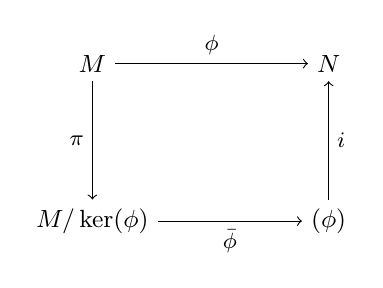
\begin{tikzpicture}[xscale=3,yscale=2]
            \small
            \node (M)  at (0,1) {$M$};
            \node (Mk) at (0,0) {$M/\ker(\phi)$};
            \node (Mi) at (1,0) {$\im(\phi)$};
            \node (N)  at (1,1) {$N$};

            \footnotesize
            \draw [->] (M)  -- node[left] {$\pi$}        (Mk);
            \draw [->] (Mk) -- node[below]{$\bar{\phi}$} (Mi);
            \draw [->] (Mi) -- node[right]{$i$}          (N);
            \draw [->] (M)  -- node[above]{$\phi$}       (N);
        \end{tikzpicture}
        \caption{First isomorphism theorem of modules.}
        \label{fig:FITModule}
    \end{figure}
    \item Example: $A=\Z$ and $M=\Z/(27)$.
    \item Theorem: Let $R$ be a PID. Then every $R$-submodule of $R^n$ is isomorphic to $R^m$ for some $0\leq m\leq n$.
    \item Think in terms of fields! If Nori had been couching all of this in terms of vector spaces, we would all get all of this immediately.
    \item Let $n=1$, $(2)\subsetneq\Z$. Then $m=n$ does not imply $M=R^n$.
    \item Submodules of $R$ are ideals. Thus, in a PID, they're principal ideals.
    \begin{proof}
        Case 1 (base case): Let $n=1$. We know that $M=(b)$ for some $b\in R$. If $b=0$, then we're done. Thus, assume $b\neq 0$. Then $T:R\to(b)$ given by $T(a)=ab$ for all $a\in A$. It follows that $T$ is onto. From the fact that $R$ is an integral domain, we have that $T$ is 1-1.\par
        Case 2 (general case): We induct on $n$. Suppose that $i:R^{n-1}\hookrightarrow R^n$ is given by
        \begin{equation*}
            i(a_1,\dots,a_{n-1}) = (a_1,\dots,a_{n-1},0)
        \end{equation*}
        Let $M$ be a submodule of $R^n$. Then $R^{n-1}\times\{0\}\hookrightarrow R^n$ and $M\cap(R^{n-1}\times\{0\})\cong R^\ell$ for $0\leq\ell\leq n-1$. Suppose that you define the ideal $\pi(a_1,\dots,a_n)=a_n$. Let $\pi(M)=I$. Then you have some ideal $I$. It follows that $\pi:M\to I\subset R$. Let $M'=\ker\phi$. $M/M'\cong I$. At this point, there are only two cases ($a=0$ and $a=M$).
    \end{proof}
    \item Next time: We will wrap up this proof with the following proposition.
    \item Proposition: If $M'$ is a submodule of $M$ and $M/M'\cong R$ as an $R$-module, then $M\cong M'\oplus R$.
\end{itemize}




\end{document}